La función objetivo se compone de varios términos, unos se muestran en la
factura de la luz, mientras que las depreciaciones las consideramos como gastos
de mantenimiento, o alquiler de los elementos de la instalación.

\begin{itemize}
	\item \textbf{Término fijo}: a pagar en función de la potencia máxima
	      contratada con la comercializadora.

	\item \textbf{Término variable}: coste de la energía neta consumida. En la
	      modalidad de autoconsumo con compensación simplificada con tarifa regulada,
	      la energía que consumimos la pagamos a precio PVPC (Precio Voluntario para el
	      Pequeño Consumidor), mientras que se nos compensa a precio de mercado diario
	      (algo menor al no incluir impuestos y comisiones). Este valor no puede ser
	      menor que cero, es decir, la comercializadora no nos pagará nunca en el caso
	      de que hayamos aportado más energía que consumido, como mucho podemos llegar
	      a tener un término variable de 0 euros. Aunque muchas comercializadoras
	      ofrecen el servicio de 'batería virtual', que se asemeja a una hucha, donde
	      si en algún mes hemos salido a ganar, la compañía nos guarda este saldo para
	      poder gastarlo en forma de consumo eléctrico en los próximos meses. En un
	      hipotético caso de superavit energético en verano y deficit en invierno, en
	      verano podríamos 'guardar' esos excedentes en la 'batería virtual' para los
	      meses de invierno.

	\item \textbf{Depreciación de equipos}: los componentes pierden valor con el
	      tiempo y el uso. Hemos aplicado una depreciación lineal, desde el coste
	      inicial función de la dimensión del equipo (dadas en el capítulo de
	      adquisición de datos), hasta el final de su esperanza de vida donde el valor
	      es nulo. Esta desvalorización se ha hecho temporal para los paneles
	      solares, depósito de agua y bomba de calor (vida útil de 20 años), y por
	      uso o tiempo para baterías y generador diesel.
\end{itemize}

a continuación consideramos tres tipos de escenarios distintos en los que solo
varía la formulación para el término variable del coste, por lo que en primer
lugar examinamos los costes fijos y depreciaciones, que son comunes a todos los
casos.

\subsection{Término fijo}

\begin{equation}
	\sum_{t=1}^{T} h \cdot C_\text{fijo}(P_\text{red,max})
\end{equation}

en el cual el coste $C_{\text{fijo}}$ por potencia máxima contratada aparece en la factura de la
luz (imagen \ref{fig:fixed_energy_cost}), y se ha establecido como $39.1 \left[\frac{\text{\euro}}{kW\cdot \text{\text{año}}}\right]$
sumando los dos términos (valle y punta).
Traducido a vatios y segundos es:

\begin{equation}
	39.1 \left[\frac{\text{\euro}}{kW\cdot \text{año}}\right] \cdot \frac{1[kW]}{1000[W]} \cdot \frac{1[\text{año}]}{(8760 \cdot 3600)[s]} = 1.239 \cdot 10^{-9} \left[\frac{\text{\euro}}{W\cdot s}\right]
\end{equation}



\begin{figure}[h] \centering
	\centering
	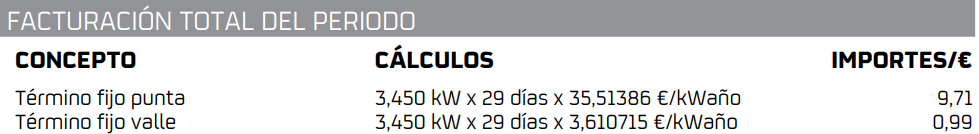
\includegraphics[width=1\textwidth]{./capitulos/resultados_discusion/images/fixed_energy_cost.png}
	\caption{Términos fijos de la factura de la luz.}
	\label{fig:fixed_energy_cost}
\end{figure}


\subsection{Depreciación de equipos}

\subsubsection{Depósito de agua caliente}

El coste del tanque es función de su volumen, y lo obtenemos de la fórmula dada
por la regresión linear del capitulo de adquisición de datos. Dividimos el coste
del tanque por el número de segundos que tiene su vida útil (20 años) para
sacar su desvalorización temporal.

Por ejemplo, para un tanque de 1000 euros:

\begin{equation}
	D_\text{tanque}(V) = \frac{1000[\text{\euro}]}{20[\text{años}]} = \frac{1000[\text{\euro}]}{(20 \cdot 8760 \cdot 3600)[s]} = 1.5854 \cdot 10^{-6} \left[\frac{\text{\euro}}{s}\right]
\end{equation}

ya que un año tiene 8760 horas y cada hora 3600 segundos.

En la función objetivo incorporamos este coste de depreciación multiplicando
por el número de segundos que tiene un paso $h$, y sumando para todos los pasos
de la simulación.

\begin{equation}
	\sum_{t=1}^{T} h \cdot D_\text{tanque}(V)
\end{equation}


\subsubsection{Paneles solares}

El coste es función de la potencia solar instalada $S$, y al igual que con el
depósito, hacemos una depreciación temporal asumiendo una vida útil de 20
años.

\begin{equation}
	\sum_{t=1}^{T} h \cdot D_\text{solar}(S)                                                                                                        \\
\end{equation}


\subsubsection{Baterías}

Coste proporcional a su capacidad ($[kW \cdot h]$).

En vez de hacer una desvalorización temporal, que resultaría demasiado
simplista, hemos modelado el desgaste de las baterías en base a su uso.

Sin penalizar la puesta en funcionamiento, resulta que podríamos estar
constantemente utilizando el acumulador como instrumento especulativo para
comprar y vender energía. Cargando y descargando varias veces por día.

Pero en realidad una batería tiene un número limitado de ciclos de funcionamiento.
Siendo un ciclo una carga hasta el máximo de capacidad y descarga hasta un
porcentaje de esta, indicado por el DoD (Depth of Discharge), como se ilustra
en la figura \ref{fig:dod_vs_cycles_lifepo4}.

Llegado a ese número de ciclos límite, las células siguen siendo funcionales,
pero su capacidad máxima ya es solo un porcentaje de la capacidad original
(e.g. 80\%). Degradadas a este punto, le damos un valor de 0 euros a las
baterías y consideramos su reemplazo.

\begin{figure}[h] \centering
	\centering
	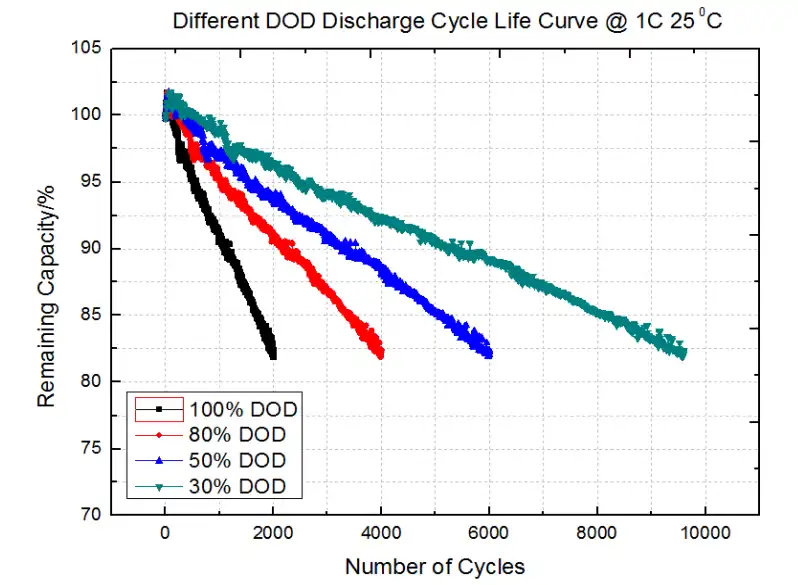
\includegraphics[width=0.8\textwidth]{./capitulos/resultados_discusion/images/dod_vs_cycles_lifepo4.png}
	\caption{Ciclos de vida de una batería LifePo4 y nivel de descarga empleado,
		con C-rate de 1. Fuente:
		\url{https://www.bravabatteries.com/lifepo4-battery-discharge-and-charge-curve/}.}
	\label{fig:dod_vs_cycles_lifepo4}
\end{figure}

Si vaciamos por completo, hasta tener una capacidad del 82.5\% de la nominal,
la cantidad de usos se menciona de 2000, mientras que si solo descargamos un
30\%, de 9500.

De forma que parece que la vida útil es función del DoD, sin embargo vamos a
tomar que la longevidad viene marcada por la máxima cantidad de energía que la
batería puede mover, independientemente de cómo la haya procesado, ya que el
producto $\text{DoD} \cdot \text{n\_ciclos}$ es similar para los distintos
modos de funcionamiento (tabla \ref{tab:DoD_results}).

\begin{table}[h]
	\centering
	\begin{tabular}{ccc}
		\toprule
		\textbf{DoD} & \textbf{n\_ciclos} & \textbf{DoD} $\cdot$ \textbf{n\_ciclos} \\
		\midrule
		1.0          & 2000               & 2000                                    \\
		0.8          & 4000               & 3200                                    \\
		0.5          & 6000               & 3000                                    \\
		0.3          & 9500               & 2850                                    \\
		\bottomrule
	\end{tabular}
	\caption{Producto del DoD y el número de ciclos con la información de la
		gráfica \ref{fig:dod_vs_cycles_lifepo4}.}
	\label{tab:DoD_results}
\end{table}


De la ficha técnica de un producto comercial, hemos extraído sus ciclos
estimados para un DoD del 70\%, hasta que su capacidad se ve reducida al
80\% de la nominal (figura \ref{fig:battery_datasheet_cycles}).

\begin{figure}[h] \centering
	\centering
	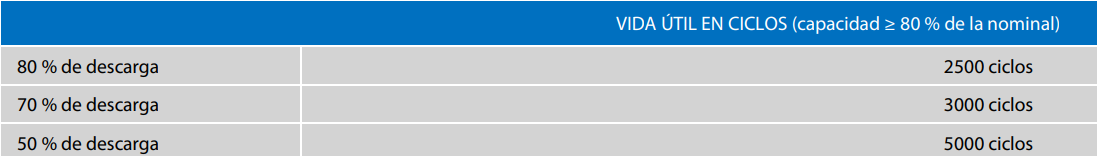
\includegraphics[width=1\textwidth]{./capitulos/resultados_discusion/images/battery_datasheet_cycles.png}
	\caption{Ciclos de vida de una batería LifePo4 y nivel de descarga empleado,
		con C-rate de 0.5. Fuente:
		\url{https://cdn.autosolar.es/pdf/fichas-tecnicas/Bat-LFP-12,8-25,6V-Smart-ES.pdf}.}
	\label{fig:battery_datasheet_cycles}
\end{figure}

Con esta información podemos calcular la energía total que puede trasegarse durante
el periodo de funcionamiento total:

\begin{equation} \label{eq:battery_life_joules}
	\text{julios} = 2 \cdot \text{ciclos} \cdot \text{DoD} \cdot e_\text{bat,max}
\end{equation}

multiplicando por dos debido a que la célula se carga y descarga en un ciclo.
Recordando que $e_\text{bat,max}$ es la capacidad.

Solo resta dividir esta cantidad del coste de las baterías para tener la depreciación
por Julio.

\begin{equation} \label{eq:battery_depreciation_by_joule}
	D_\text{bat}(e_\text{bat,max}) = \frac{\text{coste\_bat}}{\text{julios}} \left[\frac{\text{\euro}}{J}\right]
\end{equation}

Así que en la función objetivo hacemos el producto de la potencia destinada a
la batería en valor absoluto por el tiempo en segundos de un paso, para
conseguir los Julios manejados con los que obtenemos la depreciación, y
finalmente hacemos la suma para todos los pasos en el periodo de optimización $T$.

\begin{equation}
	\sum_{t=1}^{T} h \cdot |P_\text{bat}(t)| \cdot D_\text{bat}(e_\text{bat,max})
\end{equation}

No obstante surge otro problema en principio no evidente, y es que el coste por
Julio de vida útil es decreciente para la capacidad de la batería. Cuanto mayor
sea el acumulador, más económico nos resulta su uso.

Es más visible cuando en la ecuación para la depreciación
\eqref{eq:battery_depreciation_by_joule} incorporamos el valor del coste
\eqref{eq:battery_cost} y de los Julios totales en su vida estimada
\eqref{eq:battery_life_joules}.

\begin{align}
	D_\text{bat}(e_\text{bat,max}) & = \frac{\text{coste\_bat}}{\text{julios}} \nonumber                                                                                       \\
	                               & = \frac{11.87 + 611.78 \cdot e_{\text{bat\_max}}}{2 \cdot \text{ciclos} \cdot \text{DoD} \cdot e_\text{bat,max}} \nonumber                \\
	                               & = \frac{11.87}{2 \cdot \text{ciclos} \cdot \text{DoD} \cdot e_{\text{bat\_max}}} +  \frac{611.78}{2 \cdot \text{ciclos} \cdot \text{DoD}}
\end{align}

Por lo que el optimizador abusará de este fenómeno para siempre dimensionar las
baterías hasta su límite máximo.

El problema es que implícitamente estamos asumiendo que la batería durará
infinitamente en el tiempo, hasta que no se le de el uso que tiene, o se
consuman sus ciclos.

En realidad lo que queremos es el máximo entre la depreciación de la batería
por su uso, y la depreciación por tiempo.

De forma similar, la garantía para un coche eléctrico se da hasta un máximo de
años, o de kilómetros recorridos por el vehículo.

Y en nuestro caso, expresamos la depreciación como:

\begin{equation}
	\text{max} \left( \sum_{t=1}^{T} h \cdot |P_\text{bat}(t)| \cdot \text{Du}_\text{bat}(e_\text{bat,max}), \quad \sum_{t=1}^{T} h \cdot \text{Dt}_\text{bat}(e_\text{bat,max}) \right)
\end{equation}

donde hemos designado $\text{Du}$ como la depreciación por uso, $\text{Dt}$ la
depreciación por tiempo, y de estas tomamos el máximo como el coste por
depreciación.

\subsubsection{Bomba de calor}

Para la bomba de calor no tenemos claro cómo estimar su número máximo de horas
de funcionamiento, por lo que no consideramos su depreciación por uso, y
simplemente depreciamos por unidad de tiempo.

Le asignamos una vida útil de 20 años.

\begin{equation}
	\sum_{t=1}^{T} h \cdot D_\text{bomba}(S)                                                                                                        \\
\end{equation}


\subsubsection{Generador diesel}

Para el caso de una vivienda off-grid, reemplazamos la red por un generador
diesel. Y para este también hemos hecho una depreciación basada en el uso,
semejante a la bomba de calor, con una longevidad del equipo de 10 años.

Pero al igual que con las baterías, no podemos simplemente depreciar por uso, y
debemos de tomar el máximo entre la depreciación por uso y tiempo.

\begin{equation}
	\text{max} \left( \sum_{t=1}^{T} h \cdot P_\text{red}(t) \cdot \text{Du}_\text{red}(P_{red_{max}}), \quad \sum_{t=1}^{T} h \cdot \text{Dt}_\text{red}(P_{red_{max}}) \right)
\end{equation}

Aunque se trate de un grupo electrógeno, lo seguimos denominando como la red
para no modificar las ecuaciones.

Y se comporta como si fuera la red, salvo que no podemos inyectar potencia en
este.


\subsection{Coste en modalidad de autoconsumo con compensación}

\begin{equation} \label{eq:cost_regulated}
	\begin{split}
		\text{Coste\_Autoconsumo} = & \max \left(0, \sum_{t=1}^{T} h \cdot \max(\text{precio}_\text{pvpc}(t) \cdot P_{red}(t), \text{precio}_\text{diario}(t) \cdot P_{red}(t)) \right)                                      \\
		                            & + \sum_{t=1}^{T} h \cdot C_\text{fijo}(P_\text{red,max})                                                                                                                               \\
		                            & + \text{max} \left( \sum_{t=1}^{T} h \cdot |P_\text{bat}(t)| \cdot \text{Du}_\text{bat}(e_\text{bat,max}), \quad \sum_{t=1}^{T} h \cdot \text{Dt}_\text{bat}(e_\text{bat,max}) \right) \\
		                            & + \sum_{t=1}^{T} h \cdot D_\text{solar}(S)                                                                                                                                             \\
		                            & + \sum_{t=1}^{T} h \cdot P_\text{bomba}(t) \cdot D_\text{bomba}(P_\text{bomba,max})                                                                                                    \\
		                            & + \sum_{t=1}^{T} h \cdot D_\text{tanque}(V)
	\end{split}
\end{equation}

donde:

\begin{itemize}
	\item $P_{red}(t)$: potencia intercambiada con la red en el instante $t$.
	      Dada por el balance de potencias en \eqref{eq:power_balance}:

	      \begin{equation} \label{eq:p_grid}
		      P_{red} =  - P_{solar} + P_{carga} + P_{bat} + P_{bomba} + P_{sobrante}
	      \end{equation}

	\item $h$: intervalo de tiempo entre muestras.
	\item $\text{precio}_\text{pvpc}(t)$: precio de compra de electricidad (PVPC)
	      en el instante $t$.
	\item $\text{precio}_\text{diario}(t)$: precio de venta de excedentes en
	      el instante $t$.
	\item $C_\text{fijo}(P_\text{red,max})$: coste fijo por potencia máxima
	      contratada.
	\item $\text{Du}_\text{bat}(e_\text{bat,max})$: depreciación de la batería por unidad
	      de energía.
	\item $\text{Dt}_\text{bat}(e_\text{bat,max})$: depreciación de la batería por unidad
	      de tiempo.
	\item $D_\text{solar}(S)$: depreciación de los paneles solares por unidad de
	      tiempo.
	\item $D_\text{bomba}(P_\text{bomba,max})$: depreciación de la bomba de calor
	      por unidad de energía.
	\item $D_\text{tanque}(V)$: depreciación del tanque de agua por unidad de
	      tiempo.
\end{itemize}


El término variable es

\begin{equation}
	\max \left(0, \sum_{t=1}^{T} h \cdot \max(\text{precio}_\text{pvpc}(t) \cdot P_{red}(t), \text{precio}_\text{diario}(t) \cdot P_{red}(t)) \right)
\end{equation}


que interpretamos como

\begin{equation}
	\max \left(0, C_{\text{variable}}) \right)
\end{equation}

porque el coste variable mínimo es de 0 euros. Esta tarifa no permite el
beneficio económico del cliente.

Y expresamos los distintos precios de la energía (compra y venta), a través de
los signos de la potencia de red, teniendo en cuenta que el precio PVPC es
siempre mayor que el precio diario.

\begin{equation}
	C_{\text{variable}} = \sum_{t=1}^T h \cdot \max(\text{precio}_\text{pvpc}(t) \cdot P_{red}(t), \text{precio}_\text{diario}(t) \cdot P_{red}(t))
\end{equation}

Si la potencia de red es positiva (compra), aplicamos el precio PVPC, y en caso
de venta el precio diario, que es igual al de compensación de excedentes.


\subsection{Coste con compensación ilimitada}

Simplemente en la ecuación \ref{eq:cost_regulated}, eliminamos el primer $\max$
del término variable de la energía.

Se permite de esta forma el beneficio económico por la venta de excedentes.

\begin{equation} \label{eq:cost_free}
	\begin{split}
		\text{Coste\_compensacion\_ilimitada} = & \sum_{t=1}^{T} h \cdot \max(\text{precio}_\text{pvpc}(t) \cdot P_{red}(t), \text{precio}_\text{diario}(t) \cdot P_{red}(t))                                                            \\
		                                        & + \sum_{t=1}^{T} h \cdot C_\text{fijo}(P_\text{red,max})                                                                                                                               \\
		                                        & + \text{max} \left( \sum_{t=1}^{T} h \cdot |P_\text{bat}(t)| \cdot \text{Du}_\text{bat}(e_\text{bat,max}), \quad \sum_{t=1}^{T} h \cdot \text{Dt}_\text{bat}(e_\text{bat,max}) \right) \\
		                                        & + \sum_{t=1}^{T} h \cdot D_\text{solar}(S)                                                                                                                                             \\
		                                        & + \sum_{t=1}^{T} h \cdot P_\text{bomba}(t) \cdot D_\text{bomba}(P_\text{bomba,max})                                                                                                    \\
		                                        & + \sum_{t=1}^{T} h \cdot D_\text{tanque}(V)
	\end{split}
\end{equation}

\subsection{Coste para sistema off-grid}

Aquí adaptamos el coste \ref{eq:cost_free}, para sustituir la red por un grupo
electrógeno. Aunque a la potencia de este la seguimos llamando $P_{red}$, y
solo aplicamos la condición $P_{red} > 0$, ya que ahora no podemos volcar nada
de potencia, y su coste variable en $[kW\cdot h]$ viene dado por el precio del
litro de diesel, que hemos tomado de $1.5 \left[\frac{\text{\euro}}{l}\right]$.

Tenemos la ventaja de que no hay término fijo de la factura, de potencia
contratada con la comercializadora, porque no hay comercializadora en escenario
off-grid.

\begin{equation} \label{eq:cost_offgrid}
	\begin{split}
		\text{Coste\_offgrid} = & \sum_{t=1}^{T} h \cdot \text{precio}_\text{diesel} \cdot P_{red}(t)                                                                                                                    \\
		                        & + \text{max} \left( \sum_{t=1}^{T} h \cdot P_\text{red}(t) \cdot \text{Du}_\text{red}(P_{red_{max}}), \quad \sum_{t=1}^{T} h \cdot \text{Dt}_\text{red}(P_{red_{max}}) \right)         \\
		                        & + \text{max} \left( \sum_{t=1}^{T} h \cdot |P_\text{bat}(t)| \cdot \text{Du}_\text{bat}(e_\text{bat,max}), \quad \sum_{t=1}^{T} h \cdot \text{Dt}_\text{bat}(e_\text{bat,max}) \right) \\
		                        & + \sum_{t=1}^{T} h \cdot D_\text{solar}(S)                                                                                                                                             \\
		                        & + \sum_{t=1}^{T} h \cdot P_\text{bomba}(t) \cdot D_\text{bomba}(P_\text{bomba,max})                                                                                                    \\
		                        & + \sum_{t=1}^{T} h \cdot D_\text{tanque}(V)
	\end{split}
\end{equation}


\subsection{Penalización por desvío respecto a la temperatura objetivo}

Todas las funciones objetivo descritas persiguen minimizar el coste de
operación de la instalación, pero no se ha hecho mención sobre la temperatura a
la que deseamos mantener la vivienda.

En vez de incorporar este requisito en el objetivo, se introduce como una
restricción en el problema de optimización.

\begin{equation}
	T_{habitacion} > T_{objetivo}
\end{equation}

Tomándose $T_{objetivo} = 20 ^\circ C$.

Puesto que calentar la vivienda implica un gasto económico para hacer funcionar la bomba de calor,
es razonable pensar que en el óptimo la temperatura de la habitación también será la mínima posible,
esto es, de $20 ^\circ C$.

No obstante esta suposición no es del todo cierta.

Supongamos un tramo horario en el que la electricidad es barata. Aunque la
temperatura de la vivienda se encuentre próxima a los $20 ^\circ C$ deseados,
puede resultar beneficioso calentar la casa por encima de los $30 ^\circ C$, si
siguen horas donde la luz se encarece mucho, para no tener que encender la
calefacción entonces.

Este comportamiento satisface las restricciones impuestas, y minimiza el gasto, pero
no sigue el curso de acción deseado.

Para subsanar este problema, e intentar no desviarnos de la temperatura marcada para
el hogar, añadimos a las funciones objetivo un término adicional para penalizar
la diferencia entre la temperatura de la habitación y la temperatura objetivo, como:

\begin{equation} \label{eq:temperature_penalization}
	\sum_{t=1}^{T} \varepsilon \cdot (T_{habitacion} - T_{objetivo})^2
\end{equation}

donde $\varepsilon$ es un factor igual a $10^{-4}$ estimado de forma heurística
mediante prueba y error.
